\documentclass[11pt]{amsbook}

\usepackage{../HBSuerDemir}	% ------------------------

\begin{document}

% ++++++++++++++++++++++++++++++++++++++
\hPage{b2p2/389}
% ++++++++++++++++++++++++++++++++++++++

where $F, G$ are continuous.
\\
When (2) is substituted in (1), the latter reduces to
\[
	\int \int_{R'} \phi (u, v) dA'
\]

defined over a region R' in rectangular uv-system, where
\[
	\phi (u,v) = (F(u, v), G(u, v))
\]

and R', dA', are to be determined.
\\
If (2) is solved for $u, v$ in terms of $x, y$ we have
\[
	u = f(x,y), v = g(x, y)      (2')
\]
This transformation defines a mapping from rectangular xy-system to rectangular uv-system, that is, the inverse transformation (2') of (2) maps a point P{x, y) of xy-system to a point P'(u, v) in uv-system, and maps the region R to a region R'. It also maps an elementary area dA into an elementary area dA' since F, G, f, g are continuous.
\\
Taking dA' as area du dv of an elementary rectangle $P' P'_1 P'_3 P'_2$ with sides parallel tp to u- and v-axes, dA will be the area of an elementary curvilinear parallelogram $P P_1 P_3 P_2$ whose sides and vertices are mapped to the sides and vertices of $P' P'_1 P'_3 P'_2$, under (2'):
\\
\begin{figure}[htb]
	\centering
	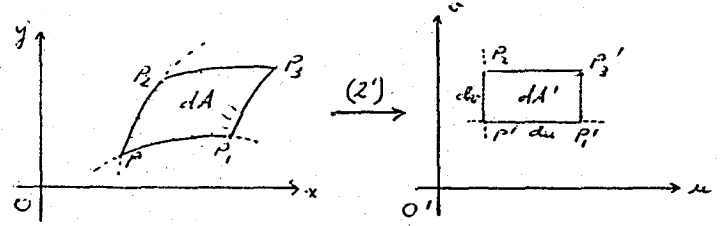
\includegraphics[width=0.9\textwidth]{images/b2p2-389-fig01}
\end{figure}
\\
Now we evaluate dA in terms of dudv.
\\
Since the curves $PP_1, PP_2$ are mapped respectively to horizontal and vertical line $P'P'_1, P'P'_2$ along which v, u are
% =======================================================
\end{document}  

%==== templates ====

%==== environments ====

%\begin{figure}[htb]
%	\centering
%	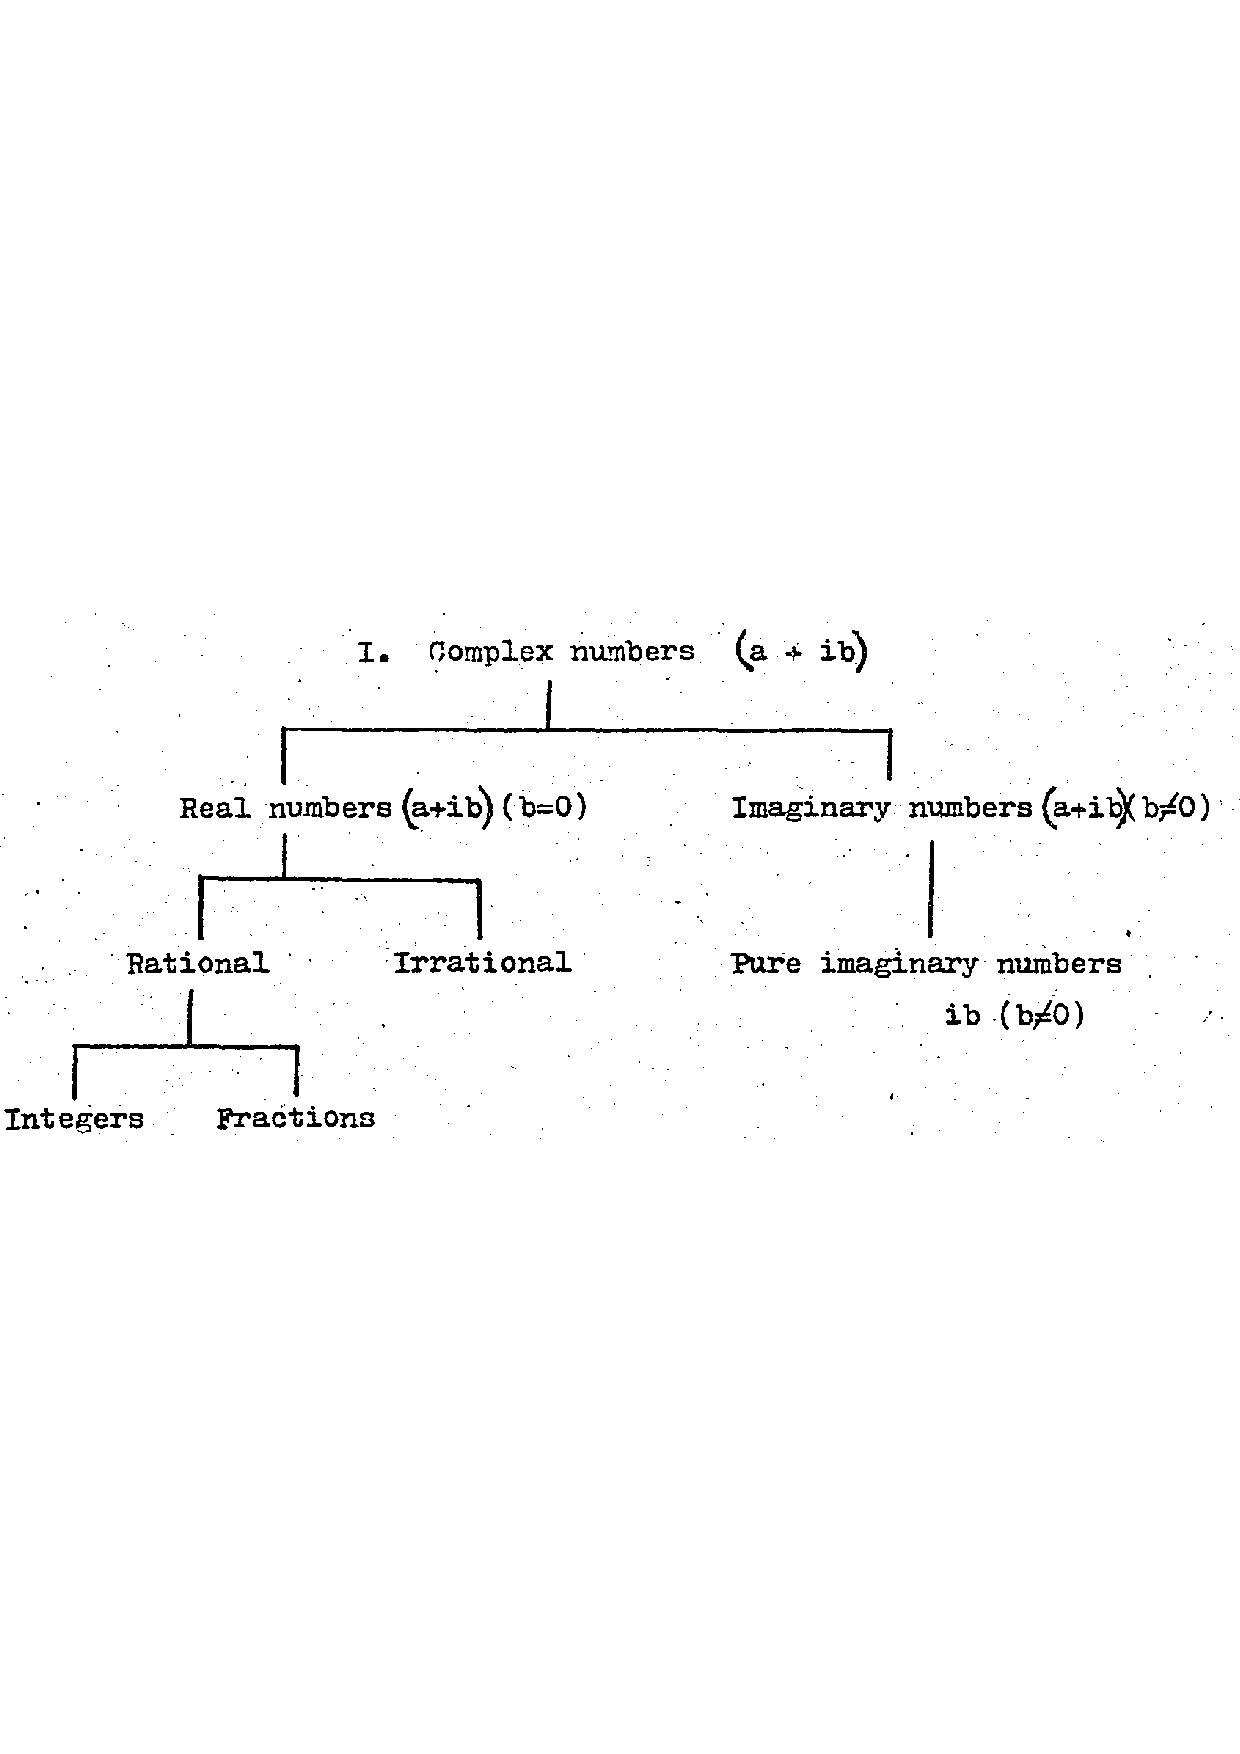
\includegraphics[width=0.9\textwidth]{images/SD-1-1p15A}
%	\caption{Classification of complex numbers}
%	\label{fig:classificationOfComplexNumbersA}
%\end{figure}

%\begin{center}
%\begin{tabular}{cc}
%\end{tabular}
%\end{center}

%\begin{exmp}
%\begin{hSolution}
%\end{hSolution}
%\end{exmp}

%\begin{hEnumerateAlpha}
%\end{hEnumerateAlpha}

%\begin{hEnumerateRoman}
%\end{hEnumerateRoman}

%$
%\begin{bmatrix}
%\end{bmatrix}
%$

%\frac{aaaa}{bbb}
%\frac{a_{n}}{b_{n}}
%\left( aaaa \right)
%\Longrightarrow

%\begin{multicols}{2}
%	bb
%\columnbreak
%	aa
%\end{multicols}
